\chapter{Výsledky}

V~předchozích kapitolách jsme již ukázali, jak vypadají vizualizace dostupnosti. Pracovali jsme však jen s~jízdními řády společnosti PID. Jak jsme však zmiňovali v~úvodu, naše aplikace má za cíl pracovat s~jízdními řády z~různých lokalit.

V~této kapitole si ukážeme, jak funguje naše aplikace pro data z~různých lokalit. Dále zmíníme, jak dlouho trvají výpočty s~jedním vstupním místem na procesoru \textbf{i5-6300U}. Pro intervalové výpočty volíme třiceti minutové okolí vstupního času s~intervalem o~délce jedné minuty.


\section{Chicago}

GTFS data pro město Chicago jsou dostupná na stránce transitfeed\footnote{Konkrétně na \url{https://transitfeeds.com/p/chicago-transit-authority/165}}.

Data jsou svou velikostí srovnatelná s~daty poskytovanými společnosti PID. Data společnosti PID obsahují zhruba 16~000~zastávek a~83~000~jízd. Data města Chicago obsahují 11~000~zastávek a~94~000~jízd.

Průměrně trvá:
\begin{itemize}
    \item Vyhodnocení dostupnosti na zastávkách: 210~ms.
    
    \item Vyhodnocení dostupnosti v~intervalu na zastávkách: 2~560~ms.
    
    \item Výpočet sousedů bodů v~rozlišení 100~x~100: 6~550~ms.
    
    \item Vyhodnocení dostupnosti pro body v~rozlišení 100~x~100: 215~ms
\end{itemize}

%odkaz na obrazky?

\begin{figure}[ht]
    \centering
    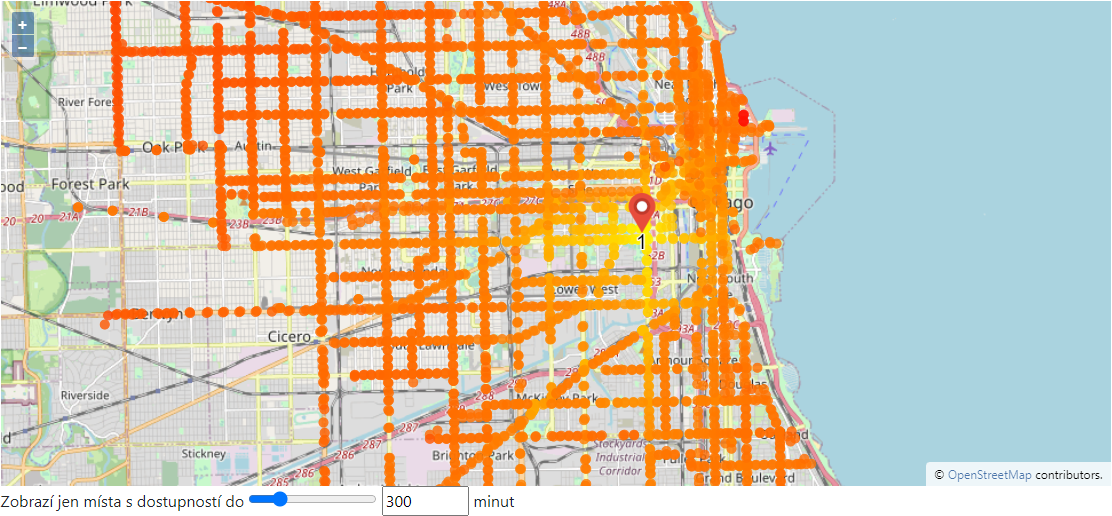
\includegraphics[width=\textwidth]{../img/Chicago-zastavky.png}
    \caption{Vizualizace dostupnosti do 300 minut na zastávkách v~Chicagu.}
    \label{fig:Chicago-zastavky}
\end{figure}

\begin{figure}[ht]
    \centering
    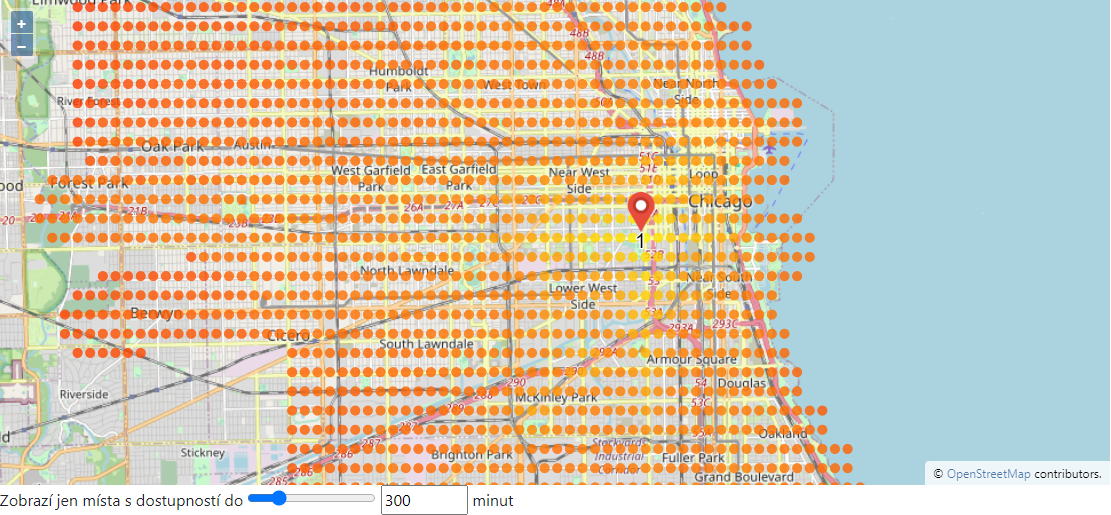
\includegraphics[width=\textwidth]{../img/Chicago-body.png}
    \caption{Vizualizace dostupnosti do 300 minut na bodech v~rastru pro Chicago.}
    \label{fig:Chicago-body}
\end{figure}


\section{Německo}

GTFS data pro celé Německo jsou dostupná na stránce \url{https://gtfs.de/en/feeds/de\_nv/}.

Jedná se o~největší jednotný dataset, který se nám podařilo nalézt. Ve srovnání s~daty společnosti PID obsahují tato data zhruba 27x~více zastávek a~16x~více jízd.

Průměrně trvá:
\begin{itemize}
    \item Vyhodnocení dostupnosti na zastávkách: 17.5~s.
    
    \item Vyhodnocení dostupnosti v~intervalu na zastávkách: 100~s.
\end{itemize}

\subsection{Problémy s~velkými daty}

Použití takto objemných dat však není jednoduché.

Zpracování a~serializace dat nám, za použití optimalizace popsané v~sekci~\ref{optim-prestupy}, trvala zhruba 2 hodiny.

Při deserializaci jsme museli navýšit maximální hloubku zanoření při čtení formátu JSON a~s~tím i~související velikost zásobníku.

Přetečení zásobníku jsme museli řešit i~na frontendu, konkrétně v~JavaScriptové funkci \textbf{Math.min}. 

Nakonec se nám podařilo vizualizovat zastávky, viz~\ref{fig:Nemecko-vse} a~\ref{fig:Nemecko-Berlin}. Pro takto velká data však naše aplikace není stavěná.

Vyhledávání je příliš pomalé pro praktické využití.

Nejsme schopni rozumně vizualizovat body v~rastru, neboť území Německa je poměrně velké a~body v~rozlišení 100~x~100 jsou vzájemně příliš vzdáleny. Větší rozlišení by vyžadovalo déle trvající předvýpočet sousedů či optimalizaci hledání sousedů.

\begin{figure}[ht]
    \centering
    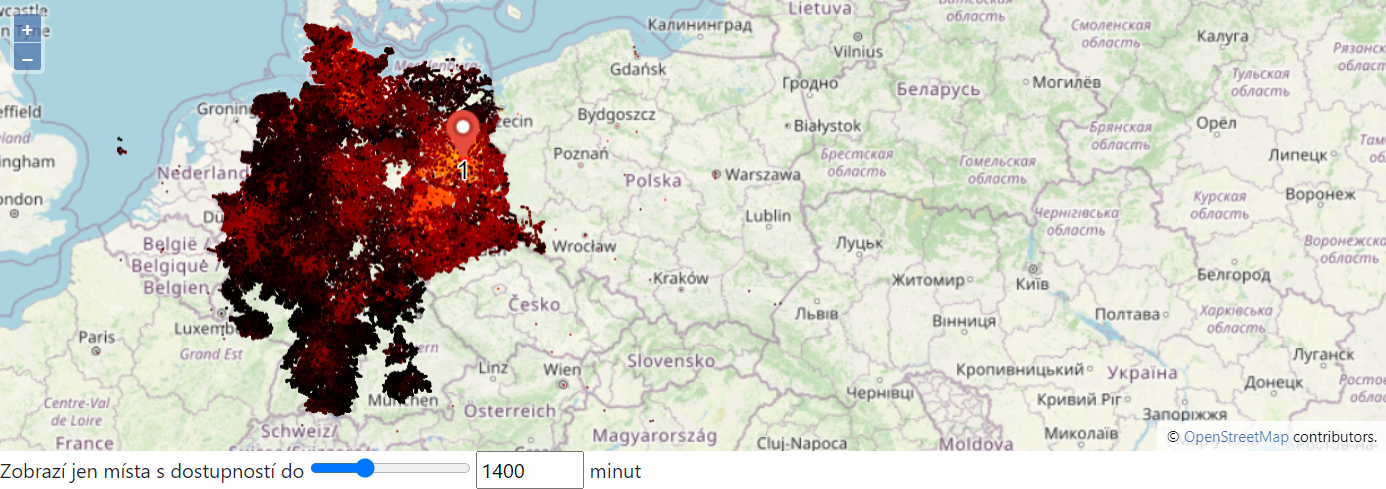
\includegraphics[width=\textwidth]{../img/Nemecko-Vse.png}
    \caption{Vizualizace dostupnosti do 1400 minut na zastávkách v~Německu.}
    \label{fig:Nemecko-vse}
\end{figure}

\begin{figure}[ht]
    \centering
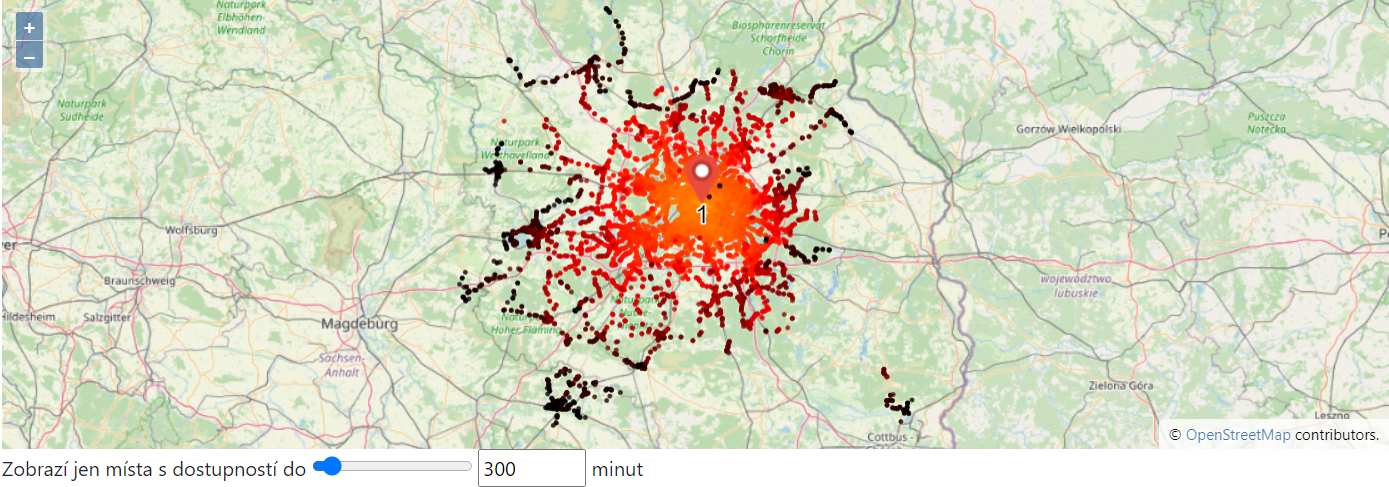
\includegraphics[width=\textwidth]{../img/Nemecko-Berlin.png}
    \caption{Vizualizaci dostupnosti do 300 minut v~okolí Berlínu.}
    \label{fig:Nemecko-Berlin}
\end{figure}